\chapter{Quantum Backflow - Basic Concepts}
%[\citealp[Ch. 2]{bar2}]
\label{chapter2}

In this chapter we start our discussion on the backflow effect. First of all, we will give an historical introduction on the first observations and subsequently we dwell into a deeper analysis. Then, we will give a rigorous definition of backflow reporting a few illustrative and relevant examples. In the central part of this chapter we will focus on outlining the basic properties of backflow in free field theories. For this purpose, we shall retrace the first work of Braken and Melloy [\citealp{bracken}], outlining its most important results and discussing in detail and rigorously their results.\\
As we remarked in Section \ref{sec:quantum_mechanincs}, considering particles of mass $m>0$, it will be convenient to work with dimensionless variables for position $x$, momentum $p$, etc., and dimensionless functions (such as the wave function $\psi$ and the current $j_\psi$) by using a length scale $\ell$ as the unit of length, $\hbar/\ell$ as the unit of momentum, $m\ell^2/\hbar$ as the unit of time, and $\hbar^2/m\ell^2$ as the unit of energy, effectively setting $m=\hbar=1$.



 %The most outstanding property that we will prove is the temporal boundedness of backflow through some point during a certain interval of time and the independence of this bound from the external parameter such as the mass of the particle and the length of the time interval. Considering particles of mass $m>0$, it will be convenient to work with dimensionless variables $x$, $p$, etc., and dimensionless functions (such as the wave function $\psi$ and the current $j_\psi$) by using a length scale $\ell$ as the unit of length, $\hbar/\ell$ as the unit of momentum, $m\ell^2/\hbar$ as the unit of time, and $\hbar^2/m\ell^2$ as the unit of energy, effectively setting $m=\hbar=1$.

\section{Historical Introduction}
Let us start by contextualizing the problem from which quantum backflow arises. Consider a particle bounded to travel freely on a straight line. According to Section \ref{sec:quantum_mechanincs}, all particles are described by a wave function $\psi(x,t)$ whose square of absolute value $|\psi(x,t)|^2$ gives the probability density of finding the particle at some point of space $x$ and at some time $t$. At the same time, if we take the Fourier transform, $\hat{\psi}(p,t)$, its square of absolute value $|\hat{\psi}(p,t)|^2$ gives the density probability of finding the particle with a given momentum $p$.\\
Suppose to shoot such a quantum particle with a given positive velocity along the straight line. Hence $\hat{\psi}(p)\neq 0$ only if $p>0$. Now consider the probability $P(t)$ of finding the particle behind a certain point, say for definiteness the origin $x=0$, at a given time $t$:
\begin{equation}
	P(t):=\int_{-\infty}^{0}\nspace\!|\psi(x,t)|^2\, \dd x
\end{equation}
Consider the following question:
\begin{verse}
	\centering
	\emph{For each wave function with strictly positive momentum, is the quantity $P(t)$ always decreasing over time?}
	\end{verse}
Classically, the answer is obvious. If you consider a particle with positive velocity, its position certainly increases with time. Instead in Quantum Mechanics, the outcome is more exotic and wave functions with positive velocity, but increasing $P(t)$ exist. This is \textit{quantum backflow}.\\
First analysis of this phenomenon date back to 1969 in a work written by Allcock [\citealp{allcock}] on the problem of time arrival as a physical observable in quantum mechanics. After that, backflow has been neglected until 1994, when Bracken and Melloy made an exhaustive investigation outlining the fundamental properties and quantitative bounds in free theory. Subsequently, Eveson, Fewster and Verch [\citealp{verch}] described backflow as a fundamental quantum inequality and in 2013 Palmero [\citealp{palmero}] gave suggestion for an experimental observation using Bose-Einstein condensate. The analysis of the results obtained by Bracken and Melloy will be discussed in this chapter while the next one will discuss mainly the study of backflow in scattering theory (particles subjected to a potential) treated in the recent work of Bostelmann, Cadamuro and Lechner [\citealp{gand}].


\section{Definition of Backflow and Illustrative Examples}
\label{sec:examples1}

The first goal of this section is to give a complete set of definitions in order to clarify the nature of backflow and the mathematics the lies behind it. We start by clarifying our notion of particles with only positive momentum by introducing the concept of \textit{right-movers}.

\begin{definition}[\textbf{Right-mover}]
	\label{def:right-mover}
	Let $\psi\in L^2(\mR)$ be a wave-function associated to a physical quantum particle and let $|\psi(x)|^2$ be the density probability. We call $\psi$ a \textit{right-mover} if $\mathrm{supp}\ \hat{\psi}\in[0,+\infty)$.
\end{definition}

\begin{oss}
	It could be seen that the set of all right-movers is a closed subspace of the Hilbert space $L^2(\mR)$. Hence, we define a projector operator which transforms each wave-function into a right-mover.
\end{oss}

\begin{definition}
	\label{def:projector_E+}
	We call $E_\pm:L^2(\mR)\to L^2(\mR)$ the operator such that:
	\begin{equation}
		\mathcal{F}[E_\pm\psi](p)=\theta(\pm p)\hat{\psi}(p)\ \forall \psi\in L^2(\mR),
	\end{equation}
	where $\theta$ is the \textit{Heaviside} function defined as:
	\begin{equation}
		\theta(p)=\begin{cases}
		0\ \ p\le 0\\
		1\ \ p>0
		\end{cases}.
	\end{equation}
\end{definition}

\begin{oss}
	This operator takes the representation of the wave-function in momentum space and removes all negative (positive in case of $E_-$) velocities. We can prove that $E_\pm$ is a real projector in the sense of the Definition \ref{def:projector}.
\end{oss}

\begin{prop}
	Let $E_+$ as in Definition \ref{def:projector_E+}. Then, $E_+$ is bounded, self-adjoint and $E_+^2=E_+$.
\end{prop}
\begin{proof}
	Boundedness is a consequence of Plancherel's Theorem. In fact, for all $\psi\in L^2(\mR)$ with $\|\psi\|=1$
	\begin{equation}
		\|E_+\psi\|=\|\mathcal{F}[E_+\psi]\|=\|\theta\hat{\psi}\|\le\|\hat{\psi}\|=\|\psi\|=1
	\end{equation}
	Self-adjointness is a by-product of the properties of the Fourier transform
	\begin{equation}
		(\psi|E_+\phi)=(\hat{\psi}|\hat{E_+\phi})=(\hat{\psi}|\theta\hat{\phi})
		=(\theta\hat{\psi}|\phi)=(E_+\psi|\phi)\ \forall \phi,\psi\in L^2(\mR),
	\end{equation}
	while $E_+^2=E_+$ holds per construction.
\end{proof}

Note that from this definition we can re-define equivalently every right-mover as those wave-functions $\psi$ such that $E_+\psi=\psi$. Henceforth, we will write the set of all right-movers with the symbol $E_+L^2(\mR)$.\\
 Once we have introduced these concepts, we are able to give an exhaustive definition of backflow:
\begin{verse}
	\centering
	\emph{Given a right-mover $\psi=E_+\psi$, backflow occurs whenever the density probability current function $j_\psi=-i/2[\psi^*\partial_x\psi-\psi\partial_x\psi^*]$ assumes negative values.}
\end{verse}
\begin{oss}
The fact that the density current assumes negative values in some point $x\in\mR$ is equivalent to the increasing of the probability of finding the particle in $(-\infty,x)$. In fact, if we set $x=0$
\begin{equation}
\begin{aligned}
\dot{P}(t)&=\frac{\dd}{\dd t}\int_{-\infty}^{0}\nspace\!|\psi(x,t)|^2\, \dd x\\
&=\int_{\infty}^{0}(\partial_t\psi(x,t)\psi^*(x,t)+\psi(x,t)\partial_t\psi^*(x,t))\, \dd x\\
&= \int_{-\infty}^{0}\nspace(-i\psi^*(x,t)H_0\psi(x,t)+i\psi(x,t)H_0\psi^*(x,t))\, \dd x\\
&=-j_\psi(0,t)\,,
\end{aligned}
\end{equation}
where we used integration by parts and the Schr\"{o}dinger equation with the Hamiltonian of free particle $H_0=P^2/2=-\partial_x^2/2$. Notice that this equation holds true also in interacting situations, where $H=H_0+V$.
\end{oss}

At this point, we are interested in showing clearly that backflow is a truly quantum effect predicted by the non-relativistic mono-dimensional Schr\"{o}dinger equation. to this avail, we will illustrate some examples in which backflow occurs.

\subsection{Superposition of Plane Waves}

The first instructive example is given by:
\begin{equation}
\begin{aligned}
&\psi(x,t)=Ae^{i\theta_1(x,t)}+Be^{i\theta_2(x,t)},\\
&\text{where}\ \theta_n(x,t)=\left[p_n\left(x-\frac{p_n t}{2}\right)+\gamma_n\right]\ n=1,2.
\end{aligned}
\label{ex1_plane_waves}
\end{equation}
Here we choose $A$, $B$, $p_1$ and $p_2$ positive constants, while $\gamma_1$ and $\gamma_2$ are arbitrary real numbers. Eq. (\ref{ex1_plane_waves}) is the sum of two plane waves, eigenfunctions of the free-particle Hamiltonian, with positive momentum $p_n$ and energy $p_n^2/2$ for $n=1,2$. This does not represent a real state because it is not normalizable. Nevertheless it could be interesting to study how backflow could emerge from such a simple case. In fact, we can evaluate the density probability current $j_\psi(x,t)$ at a certain point $x\in\mR$ and at the instant $t\in\mR$. Remembering Definition \ref{def:density_current} for $j_\psi(x,t)$ we obtain:
\begin{equation}
\begin{aligned}
& j_\psi(x,t)=A^2p_1+B^2p_2+AB(p_1+p_2)\cos(\theta_1(x,t)-\theta_2(x,t)).
\end{aligned}
\end{equation}
We can check that $\theta_1(x,t)-\theta_2(x,t)$ is linearly dependent with the time $t$. Hence the density current could vary from an upper value of $(p_1A+p_2B)(A+B)$ to a lower value of $(p_1A-p_2B)(A-B)$. If, for example $A>B$ and $p_1A<p_2B$, this lower value is negative and so backflow occurs.\\ %In fact if we set the parameters to be
%\begin{equation}
%p_1=0.3,\ p_2=1.4,\ \gamma_1=0,\ \gamma_2=0,\ A=1.8,\ B=1
%\end{equation}
%and plot the corresponding $j_\psi$ in Figure (), we see clearly that for some intervals the density current is negative.\\
%\begin{figure}[h]	
%	\centering
%	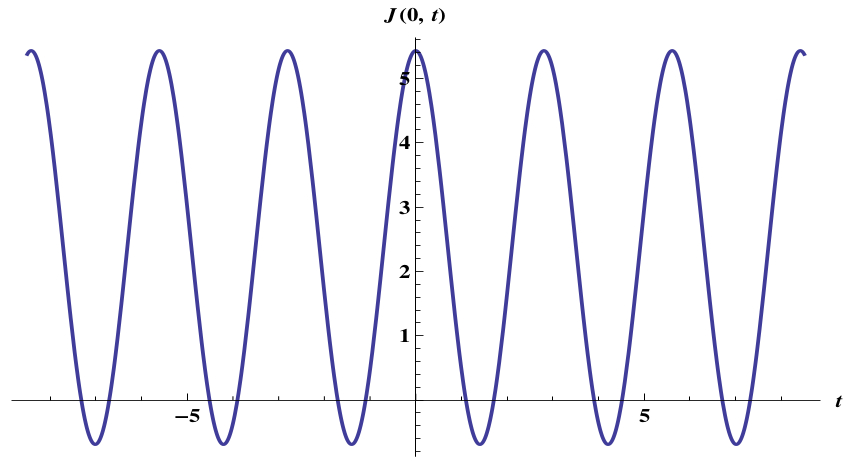
\includegraphics[scale=0.25]{images/plane_wave}
%	\caption{as}
%	\label{fig:plane_wave}
%\end{figure}
Although this example has no physical interpretation, because of the non-normalizability of plane waves, we can note that backflow is essentially an interference effect between some wave-packets with high positive momentum and others with low positive momentum. This aspect is not trivial and we will we re-use it for proving an important theorem regarding the intensity of backflow through a single point at a some instant of time. In particular, we will construct a normalized wave-packet in momentum space as a sum of a function $\tilde{\chi}(p)\in L^2(\mR_+)$ and its translation $\tilde{\chi}(p-n)$, with $n\in\mathbb{N}$. This coincides with taking the interference of two wave-packets with different positive momenta.

\subsection{Superposition of Gaussian Wave-packets}
\label{sec:gaussian}
Another example can be made by replacing the two plane waves with Gaussian functions tightly picked in momentum. This represents a more physically realistic state. We consider the sum of two initial Gaussian wave-packets with equal
spatial width $\sigma$, evolved for a time $t$. The corresponding normalized wave function is
\begin{multline}
	\psi(x,t)=\sum_{n=1,2}C_n\frac{1}{\sqrt{4\sigma^2+2it}}\exp\left(ip_n(x-p_nt)-\frac{(x-p_nt)^2}{4\sigma^2+2it}\right),\\ \ C_n\in\mR,\ p_1,p_2>0.
\end{multline}
This function was proposed by Yearsley in [\citealp{years}]. As in the previous example, this wave-function is given by the superposition of two waves with different momentum. Note that as $\sigma\to0$, we obtain once more a superposition of plane waves. To prove that for such a function backflow occurs, we set the parameters $p_1,p_2,C_1,C_2$ and $\sigma$ to be
\begin{equation}
\label{eq:parameters}
p_1 = 0.3, \ p_2 = 1.4,\ C_1 = 1.8,\ C_2 = 1,\ \sigma= 10.
\end{equation}
We plot the probability $P(t)$ of the particle being localized at a point $x < 0$ as a function of time, see Figure \ref{fig:back_2}. Observe that $P(t)$ is non monotonically decreasing, but in several disjoint time intervals it increases, proving the presence of backflow.

\begin{figure}[h]	
\centering
\begin{minipage}{0.45\textwidth}
		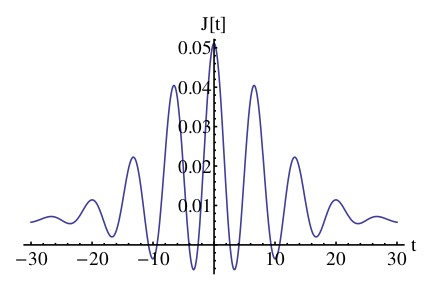
\includegraphics[scale=0.43]{images/gaussian_1}
		\caption{Plot of the current for a superposition of
			two gaussians, with the parameters given in Eq. [\ref{eq:parameters}].}
		\label{fig:back}
\end{minipage}
\hfil
\begin{minipage}{0.45\textwidth}
		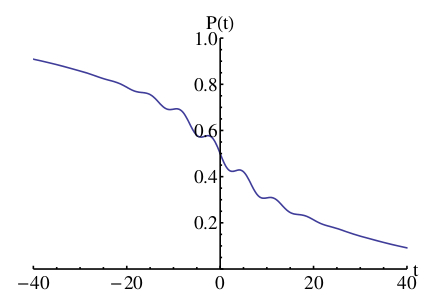
\includegraphics[scale=0.43]{images/gaussian_2}
		\caption{Plot of the probability for
			remaining in $x < 0$ for a superposition of two gaussians,
			with the parameters given in Eq. [\ref{eq:parameters}]. }
		\label{fig:back_2}
\end{minipage}
\end{figure}
One might wonder how to quantify the amount of backflow that this state displays. To answer this query, we need to evaluate
\begin{equation}
	P(t_1)-P(t_2)=\int_{t_1}^{t_2}\nspace\!j_\psi(0,t)\, \dd t,
	\label{eq:prob_flux}
\end{equation} 
where $P$ is the probability of finding the particle within the domain $x<0$ while $[t_1 , t_2 ]$ is the interval maximizing the amount of backflow for this wave-function. A direct evaluation shows that,
\begin{equation}
	F:=\mathrm{inf}\{P(t_1)-P(t_2)\ |\ t_2>t_1 \}\approx -0.0061
\end{equation}
We will see in the following discussion that this flux is approximately the 16\% of the maximum amount of backflow theoretically allowed. 
\subsection{Normalizable Wave}

The following example shows that backflow can also occur for normalizable wave-functions. Let us consider $\phi\in L^2(\mR)$ whose representation in the momentum space (which is nothing more than its Fourier transform $\hat{\phi}$) is given by the following equation:
\begin{equation}	
	\hat{\phi}(p)=\begin{cases}
	\frac{18}{\sqrt{35K}}p(e^{-p/K}-\frac{1}{6}e^{-p/2K}) & p>0\\
	0 & p\le 0
	\end{cases}
	\label{ex2:def}
\end{equation}
where $K$ is a positive constant. This represents a possible initial state for a physical particle. Now we can write the expression for the function $\phi$ defined in the position space:
\begin{equation}
\begin{aligned}
	&\phi(x)=18\sqrt{\frac{K}{70\pi}}\left[\frac{1}{(1-iKx)^2}-\frac{2}{3(1-2iKx)^2}\right].
\end{aligned}\label{ex2:position}
\end{equation}
At this point we can evaluate $\phi(0)$, $\phi'(0)$ and the density probability current $j_\phi(0)$ as:
\begin{equation}
\begin{aligned}
&\phi(0)=6\sqrt{\frac{K}{70\pi}} & \phi'(0)=-12i\sqrt{\frac{K}{70\pi}}\\
& j_\phi(0)=-\frac{36K^2}{35\pi }<0,
\end{aligned}
\end{equation}
which proves the presence of backflow. Evaluating the time evolution of this wave-function, the current is negative during the interval $[0,t_1]$ where $t_1 \approx 0.021/K^2$. The corresponding flux, from (\ref{eq:prob_flux}), is
\begin{equation}
	F\approx-0.0043
\end{equation}

\section{Backflow in Free Theory}
In this section we want to study the length and the strength of this effect in the case of free particles. In particular, The question we ask ourselves is:
\begin{verse}
	\centering
\emph{What is the maximum amount of probability which could flow back through a point $x_0$ during an interval of time $T$ for a right-moving free-particle?}
\end{verse}
We will show that this problem is equivalent to finding the smallest eigenvalue of a suitable integral operator, out of which one establish a bound for quantum backflow.\\
In the following discussion we will interpret the flux of probability defined in Eq. (\ref{eq:prob_flux}) in a time interval $[0,T]$ through a certain point, say the origin $x=0$, as a scalar product of the form $(\hat{\psi}|\theta B_T \theta \hat{\psi})$, where $\hat{\psi}$ is the Fourier transform of the wave-function (i.e. right-mover), $\theta$ is the Heaviside function and $B_T$ is the \textit{backflow operator} that will be proved to be bounded and self-adjoint. After that, we will link the upper bound for this operator to the evaluation of the maximum eigenvalue of an integral operator $K$ (defined by Bracken and Melloy in [\citealp{bracken}]). Furthermore, we will show that this maximum eigenvalue corresponds to the maximum amount of backflow allowed for any right-mover. In this part of our thesis will report the results obtained by Penz \textit{et al.} in [\citealp{penz}].\\
\subsection{Temporal Boundedness of Backflow}
Let us start by considering how the free Schr\"{o}dinger evolution operator acts in momentum space. We have shown in Section \ref{sec:quantum_mechanincs} that for a wave-function represented in the Fourier-transformed space $\hat{\psi}$, the evolution operator $U_t$ could be transformed into a phase multiplicative operator:
 \begin{equation}
 	\hat{\psi}_t(p)=\widehat{U_t\psi}=(\widehat{U}_t\hat{\psi})(p)=e^{-ip^2t/2}\hat{\psi}(p)\, ,
 	\label{eq:unitary_evolution}
 \end{equation}
 where we introduced the operator $\widehat{U}_t:=\mathcal{F}U_t\mathcal{F}^{-1}$.
 
 \begin{oss}
 	Notice that, if $\psi\in E_+L^2(\mR)$, then, by definition of $\widehat{U}_t$, $U_t\psi\in E_+ L^2(\mR)$ for all $t\in\mathbb{R}$. Stated differently, the evolution preserves the subspace $E_+L^2(\mR)$ of right-mover wave-functions. Furthermore, we observe that $U_t^*=U_{-t}$ and $\widehat{U}_t^*=\widehat{U}_{-t}$. 
 	\label{oss:widehat(U)}
 \end{oss}
  The representation of such wave-functions in the "position" space are given by the anti-Fourier transform:
\begin{equation}
\psi_t(x)=\frac{1}{\sqrt{2\pi}}\int_{-\infty}^{+\infty}\nspace\! e^{ipx}\hat{\psi}_t(p)\, \dd p.
\end{equation}
Let a particle be described in momentum space by a wave-function $\hat{\psi}(p)$ at time $0$. If $\|\hat{\psi}\|=\|\psi\|=1$, the probability that a position measurement at time $t$ yields a position $x > 0$ reads
\begin{equation}
	L(\psi_t):=\int_{0}^{+\infty}\nspace\!|\psi_t(x)|^2\, \dd x=(\hat{\psi}|\widehat{U}^*_t\mathcal{F}\theta\mathcal{F}^{-1} \widehat{U}_t\hat{\psi}).
\end{equation}
Now we restrict to consider right-moving wave-functions $\psi$ such that $E_+\psi=\psi$ or equivalently $\theta\hat{\psi}=\hat{\psi}$ and $\|\psi\|=1$. Note that for such functions the evolution $\psi_t$ is also a right-mover, $\psi_t=E_+\psi_t$.\\
 As shown in the previous examples, there exist right-moving wave-functions in which backflow occurs and the probability $L(\psi_t)$ does decrease in a time interval. So, it is convenient to define the maximum backflow for a fixed right-mover $\psi$ as
\begin{equation}
	\lambda(\psi)=\sup\{L(\psi_s)-L(\psi_t)\ |\ s,t\in\mR,\ t>s \}
	\label{eq:lambda_psi}
\end{equation}
Since we are interested in the maximum amount of probability backflow, we define the \textbf{backflow constant} $\lambda$ as
\begin{equation}
	\lambda:=\sup\{\lambda(\psi)\ |\ \psi=E_+\psi,\ \|\psi\|=1 \}.
	\label{eq:backflow_const}
\end{equation}
Introducing the orthogonal projector $\tilde{\theta}_t:=\widehat{U}^*_t\mathcal{F}\theta\mathcal{F}^{-1} \widehat{U}_t$ we obtain for any normalized wave-function $\psi\in L^2(\mR)$
\begin{equation}
	L(\psi_s)-L(\psi_t)=(\hat{\psi}|(\tilde{\theta}_s-\tilde{\theta}_t)\hat{\psi}).
\end{equation}
Since
\begin{equation}
	\tilde{\theta}_s-\tilde{\theta}_t=\widehat{U}^*_{\frac{t+s}{2}}(\tilde{\theta}_{\frac{s-t}{2}}-\tilde{\theta}_{\frac{t-s}{2}})\widehat{U}_{\frac{t+s}{2}},
\end{equation}
we can write
\begin{equation}
	\lambda=\sup\{  (   \hat{\psi}  |  \widehat{U}^*_{\tau}(\tilde{\theta}_{-T}-\tilde{\theta}_{T})\widehat{U}_{\tau}\hat{\psi}) \ |\ \psi=E_+\psi,\ \|\psi\|=1,\ \tau\in\mR,\ T>0\},
\end{equation}
\begin{definition}
	Given a fixed time $T>0$, we call \textbf{backflow operator} $B_T:L^2(\mR)\to L^2(\mR)$
	\begin{equation}
		B_T:=\tilde{\theta}_{-T}-\tilde{\theta}_T.
		\label{eq:backflow_operator}
	\end{equation}
\end{definition}
$B_T$ enjoys the following properties
\begin{prop}
	\label{prop:backflow_operator}
	The operator $\theta B_T\theta$ with $B_T$ defined in (\ref{eq:backflow_operator}) is bounded and self-adjoint.
\end{prop}
\begin{proof}
	The boundedness of $\theta B_T\theta$ follows from the boundedness of $\theta$ and $\widehat{U}_T$ forall $T\in\mR$. One can prove self-adjointness by considering the scalar product $(\psi|\theta B_T\theta \phi)$ for some $\psi,\phi\in L^2(\mR)$ and see that it is equal to $(\theta B_T\theta\psi|\phi)$ using self-adjointness of $\theta$ and the definition of adjoint for $\widehat{U}_T$.
\end{proof}

\begin{oss}
	Note that the operator $\theta$ here needs to cut the negative momenta of a wave-function transforming it into a right-mover.
\end{oss}

Focusing on the analysis of the backflow constant $\lambda$, since $\widehat{U}_\tau$ preserves the set of right-movers $E_+(L^2)$, see Observation \ref{oss:widehat(U)}, it holds
\begin{equation}
	\lambda=\sup\{(\phi|\theta B_T\theta \phi)\ |\ \phi\in L^2(\mR),\ \|\phi\|=1,\ T>0 \},
\end{equation} 
or equivalently 
\begin{equation}
	\lambda=\sup\bigcup_{T>0}\sigma(\theta B_T\theta).
	\label{eq:lambda_sum}
\end{equation}

\begin{oss}
	(\ref{eq:lambda_sum}) could be simplified by neglecting the set sum over $T>0$. In fact we see that $\theta B_T\theta$ is the operator which gives the flux of probability through the origin $x=0$ for a time interval $[0,T]$. Using scaling arguments, one shows that backflow is independent from the time $T$, in the sense that, for every right-mover with some amount of backflow during the interval $[0,T]$, there exists another right-mover with the same backflow, but for a time interval $[0,T']$ arbitrarily larger.
\end{oss}

\begin{prop}
	For any fixed time $T>0$, $\lambda=\sup \sigma(\theta B_T\theta)$.
	\label{prop:time_independence}
\end{prop}
\begin{proof}
	Consider the family of unitary operators $V_\mu:L^2(\mR)\to L^2(\mR) $ with $\mu>0$ defined as $(V_\mu\phi)(p):=\sqrt{\mu}\phi(\mu p)$. For any $\phi\in L^2(\mR)$
	\begin{equation}
		(\theta V_\mu \phi)(p)=\sqrt{\mu}\theta(p)\phi(\mu p)=\sqrt{\mu}\theta(\mu p)\phi(\mu p)=(V_\mu\theta\phi)(p),
	\end{equation}
	and
	\begin{equation}
		\mathcal{F}\theta\mathcal{F}^{-1}V_\mu\phi=\mathcal{F}\theta V_{1/\mu}\mathcal{F}^{-1}\phi=\mathcal{F} V_{1/\mu}\theta\mathcal{F}^{-1}\phi=V_\mu	\mathcal{F}\theta\mathcal{F}^{-1}\phi.
	\end{equation}
	Then $V_\mu$ commutes with both the operator $\theta$ and $	\mathcal{F}\theta\mathcal{F}^{-1}$. Note that $V_\mu^*=V_{1/\mu}$. A direct calculation shows that
	\begin{equation}
		V_\mu \widehat{U}_t V_\mu^*= \widehat{U}_{\mu^2t}
	\end{equation}
	It follows that
	\begin{equation}
		V_\mu\theta B_T \theta V_\mu^*=\theta B_{\mu^2T}\theta.
	\end{equation}
	Since the spectrum of an operator is invariant under a unitary transformation we have for any $T_1,T_2>0$
	\begin{equation}
	\sigma(\theta B_{T_1}\theta)=\sigma(V_{\mu'}\theta B_{T_1} \theta V_{\mu'}^*)=\sigma(\theta B_{T_2}\theta)\ \text{ where } \ \mu'=\sqrt{T_2 / T_1}.
	\end{equation}
    Hence we can write $\lambda=\sup\sigma(\theta B_{T_1}\theta)$ for any fixed $T>0.$
\end{proof}

Summing up all results we obtained for the backflow operator $B_T$ and for the backflow constant $\lambda$, it holds.

\begin{theorem}[\textbf{Temporal Boundedness of Backflow}]
	\label{th:temp_bound}
	Let $\lambda=\sup \sigma(\theta B\theta)$, where $B=B_{T=1}$ is the backflow operator. For any right-mover $\psi\in L^2(\mR)$ such that $\psi=E_+\psi$ and for any $T>0$ it holds 
	\begin{equation}
		\int_{0}^{T}\nspace\!j_\psi(0,t)\, \dd t\ge -\lambda>-\infty.
	\end{equation}
\end{theorem}
\begin{proof}
	Since $\lambda$ is the maximum amount of backflow, we must to prove that it is finite. Since the operator $\theta B\theta$ is bounded and self-adjoint (in view of Proposition \ref{prop:backflow_operator})
	\begin{equation}
		\sigma( \theta B\theta) \subseteq [-\|B\|,\|B\|].
	\end{equation}
	Hence the sought thesis descends.
\end{proof}

Once we proved temporal boundedness of backflow for free particles, we are interested about evaluating numerically the backflow constant $\lambda$ introducing the integral operator first founded by Bracken and Melloy in [\citealp{bracken}]. These authors heuristically introduce $\lambda$ via time integrals of currents at point $x = 0$ over arbitrary finite intervals, motivating their definition of $\lambda$ as the supremum of the spectrum of such integral operator.

\begin{prop}
	\label{prop:bracken_int}
	Let $K:L^2(\mR_+)\to L^2(\mR_+)$ be the integral operator:
	\begin{equation}
	\label{eq:bracken_int}
		(Kf)(u)=-\frac{1}{\pi}\int_{0}^{\infty}\frac{\sin(u^2-v^2)}{u-v}f(v)\, \dd v \ \ \forall f\in L^2(\mR_+).
	\end{equation}
	Then $\theta B\theta f  = Kf$ for all $f\in L^2(\mR_+)$. 
\end{prop}
\begin{proof}
	Since $\theta B \theta$ is bounded we only need to prove that $\theta B\theta  = K$ holds on a dense subspace of $L^2(\mR_+)$. Hence, we choose $\mathcal{S}(\mR_+):=\theta\mathcal{S}(\mR)$, i.e. the set of Schwartz functions projected with the Heaviside function.\\% the space of all smooth functions, rapidly decreasing and with support contained in $\mR_+$.\\
	First of all, we relate the orthogonal projection $\mathcal{F} \theta \mathcal{F}^{-1}$ to the Hilbert transform
	\begin{equation}
		\begin{aligned}
		& H:L^2(\mR)\to L^2(\mR), & (Hf)(p)=\frac{1}{\pi}PV\nspace\int_{-\infty}^{\infty}\frac{f(q)}{p-q}\, \dd q.
		\end{aligned}
	\end{equation} 
	Here $PV$ indicates the principal value. For $f\in\mathcal{S}(\mR)$ we obtain by means of Lebesgue's dominated convergence theorem and by means of Sochozki's formula ,see [\citealp[Example 3.3.1]{blanch}],
	\begin{equation}
		\begin{aligned}
		(\mathcal{F} \theta \mathcal{F}^{-1}f)(p) &= \frac{1}{2\pi}\int_{0}^{\infty}\nspace\!e^{-ipx}\left(\int_{-\infty}^{\infty}\nspace\!e^{ixq}f(q)\, \dd q\right)\, \dd x\\
		&= \frac{1}{2\pi}\lim_{\varepsilon\to 0^+}\int_{-\infty}^{\infty}\nspace\!f(q)\left(\int_{0}^{\infty}\nspace\!e^{i(q-p)x-\varepsilon x}\, \dd x\right)\, \dd q\\
		&= -\frac{1}{2\pi i}\lim_{\varepsilon\to 0^+}\int_{-\infty}^{\infty}\frac{f(q)}{q-p+i\varepsilon}\dd q\\
		&= -\frac{1}{2\pi i}\left\{ PV\nspace\int_{-\infty}^{\infty}\frac{f(q)}{q-p}\, \dd q-i\pi f(p)\right\}\\
		&= \frac{1}{2i}(Hf)(p)+\frac{f(p)}{2}.
		\end{aligned}
	\end{equation}
	Hence, we have 
	\begin{equation}
	\label{eq:backflow_hilbert}
		\mathcal{F} \theta \mathcal{F}^{-1}=\frac{1}{2}(-iH+\mathbb{I}).
	\end{equation}
	Now consider the backflow operator defined as $B=U\mathcal{F} \theta \mathcal{F}^{-1}U^*-U^*\mathcal{F} \theta \mathcal{F}^{-1}U$, where $U:=\widehat{U}_{T=1}$ is the unitary evolution operator in momentum space defined in (\ref{eq:unitary_evolution}). Substituting (\ref{eq:backflow_hilbert}) into the last equation, we obtain
	\begin{equation}
		B=\frac{1}{2i}(UHU^*-U^*HU).
	\end{equation}
	From this we have for $p>0$ and $\phi\in \mathcal{S}(\mR_+)$
	\begin{equation}
	\begin{aligned}
	(\theta B\theta \phi)(p)&=\frac{e^{-ip^2}}{2i}(HU^*\phi)(p)-\frac{e^{ip^2}}{2i}(HU\phi)(p)\\
	&= \frac{1}{2\pi i}\int_{0}^{\infty}\frac{e^{-i(p^2-q^2)}-e^{i(p^2-q^2)}}{p-q}\phi(q)\, \dd q\\
	&= -\frac{1}{\pi}\int_{0}^{\infty}\frac{\sin(p^2-q^2)}{p-q}\phi(q)\dd q=(K\phi)(p).
	\end{aligned}	
	\end{equation}
	Thus the restriction of $\theta B\theta \phi$ to $L^2(\mR_+)$ coincides with $K$.
\end{proof}
\begin{oss}
	With the last proposition we proved that searching the maximum amount of backflow for any right-movers is equivalent to finding the supremum of the spectrum of a suitable integral operator. Furthermore, we have that for a generic right-mover $\psi=E_+\psi$ with $\|\psi\|=1$
	\begin{equation}
	L(\psi_{t=0})-L(\psi_{t=1})=(\hat{\psi}|K\hat{\psi}),
	\end{equation}
	where $L(\psi_t)$ is the probability of finding the particle in $x>0$ at the time $t$, and $K$ the operator defined in Proposition \ref{prop:backflow_operator}.
\end{oss}

\subsection{Maximum Backflow Approximation}
	As we proved in Theorem \ref{th:temp_bound}, there exists a lower bound for backflow. To wit, for every time interval $[0,T)$ the maximum amount of probability which could flow back for a generic right-mover is always less than $|\lambda|$. We have no information concerning $\lambda$ and its eigenfunction $\phi_\lambda$. To solve this quandary, we need to study the integral operator $K$. Unfortunately, no analytical value for $\sup \sigma(K)$ is known, and numerical methods have been used to estimate $\lambda$. \\
	More precisely, we approximate $\mR_+\times\mR_+$ by $[0,N\tau]\times[0,N\tau]$ divided into a grid of $N^2$ squares of area $\tau^2$. In each square we approximate the kernel of the integral operator as a constant. At the same time we approximate the eigenfunction $\phi_{\lambda}$ as a vector $\varphi_\lambda^i$ in $\mC^n$ by considering the function constant in each interval $[i\tau,(i+1)\tau]$ with $i=1,...,n$.\footnote{see [\citealp[Sect. 5]{bracken}]} In this way we are converting our eigenvalue-problem to a linear equation:
	\begin{equation}
		-\frac{1}{\pi}\int_{0}^{\infty}\frac{\sin(u^2-v^2)}{u-v}\varphi(v)\, \dd v=\lambda\varphi(u) \stackrel{\approx}{\longmapsto} K_k^i\varphi_\lambda^k=\lambda\varphi_\lambda^i,
		\label{eq:eigenvalue_approx}
	\end{equation}
	where $K_k^i$ is the hermitian matrix obtained by approximating our integral kernel. The second equation admits a solution. In order to find a good estimate for $\lambda$ we need to take $N\to\infty$ and $\tau\to0$. Here we report some results obtained by Braken and Melloy in their work considering $\tau=0.05$. The estimates obtained are:
	\begin{center}
		\centering
		\footnotesize
		\begin{tabular}{|c|cccc|}
			\toprule
			$N$ & 100 & 200 & 275 & 500\\
			\midrule
			$\lambda$ & 0.0256 & 0.0297 & 0.0309 & 0.0323\\
			\bottomrule
		\end{tabular}
		%\caption{Estimation of maximum backflow via grid approximation}
	\end{center}
	which are apparently converging to $\lambda_{0.05}\approx0.034$. Taking smaller values of $\tau$ and letting $N\to\infty$ we obtain the estimates $\lambda_{0.04}\approx0.035$, $\lambda_{0.025}\approx0.036$ and $\lambda_{0.01}\approx0.038$.\\% Recent research had been calculated numerically with more accuracy over the years the eigenvalue $\lambda$ and estimates it to be $\approx-0.0384517$.
	
	A possible method to compute the maximum eigenvalue $\lambda$ is given by Penz in [\citealp{penz}]. It is based on an algorithm called \textit{power iteration} and it works as follows.\\
	Let $A\in\mC^{N\times N}$ be a symmetric matrix and let $a$ be the eigenvalue of $A$ with the largest absolute value. Then, consider a vector $v_0\in\mC^N$ such that $v_0\neq0$ and there is a non-zero component within the eigenspace of $A$ corresponding to $a$. Then the sequence $\{v_n\}_{n\in\mathbb{N}_0}$ recursively defined by
	\begin{equation}
		v_{n+1}=\frac{Av_n}{\|v_n\|}
	\end{equation}
	converges to a normalized eigenvector of $a$. In addition, it holds\footnote{see [\citealp[Sect. 7.3.1]{matrix}]}
	\begin{equation}
		a=\lim_{n\to\infty}v_{n+1}^\dagger\frac{v_n}{\|v_n\|}.
	\end{equation}
	
	Since $\sigma(\theta B \theta)=\sigma(K)\subset[-1,\lambda]$, the power method can be applied to the non negative, discretized operator $\theta B\theta+\mathbb{I}$. Its largest eigenvalue then approximates $\lambda +1$ while the sequence $v_n$ tends to the maximizing eigenvector.\\
	Penz started his calculations by covering a square $[0,q_0]^2$ with $N_0$ grid points and subsequently he repeated the computations for up to $N=N_0h$ grid points and a larger square $ [0,q]^2$ with $q=q_0\sqrt{h}$ for $h=1,2,$ etc.. With this method, we can at the same time make the square growing and the absolute step size getting smaller. This leads to a sequence of eigenvalues $\lambda_h$ as a function of the factor of accuracy $h$ which are used to extrapolate to $h\to\infty$ and getting an approximation $\lambda_\infty$ of the backflow constant. The results obtained by Penz are plotted in figure \ref{fig:backflow_approx_1} and \ref{fig:backflow_approx_2}.\\
	\begin{figure}[h]	
		\centering
		\begin{minipage}{0.45\textwidth}
			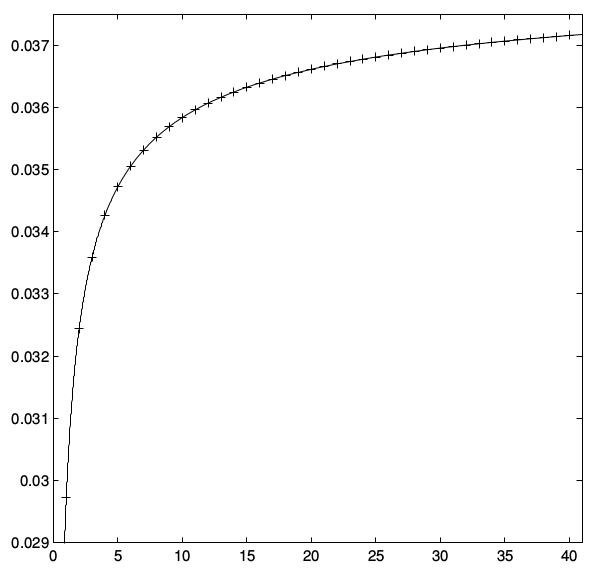
\includegraphics[scale=0.31]{images/backflow_approx_1}
			\caption{$\lambda$ plotted against $h$ and fit $\lambda_\infty+b/\sqrt h$.}
			\label{fig:backflow_approx_1}
		\end{minipage}
		\hfil
		\begin{minipage}{0.45\textwidth}
			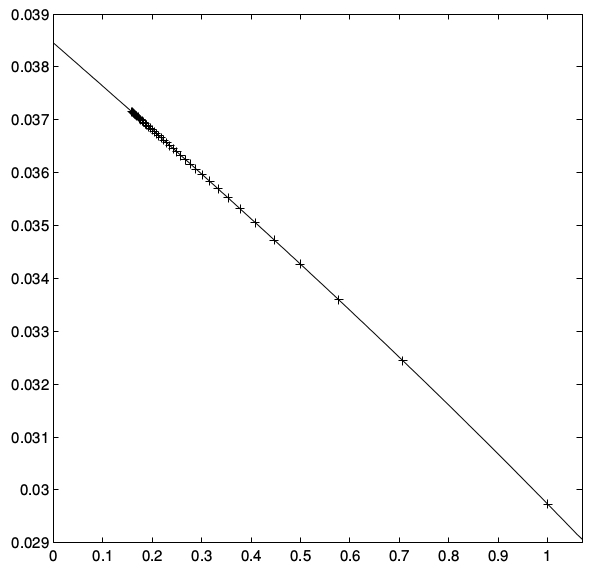
\includegraphics[scale=0.31]{images/backflow_approx_2}
			\caption{$\lambda$ plotted against $1/\sqrt h$ and polynomial fit of third order.}
			\label{fig:backflow_approx_2}
		\end{minipage}
	\end{figure}
	
	The approximation for the backflow constant can be read off from the intersection of the $y$-axis with the graph in (\ref{fig:backflow_approx_2}). This yields
	\begin{equation}
		\lambda\approx\lambda_\infty\approx 0.0384517.
	\end{equation}
	This is the final result computed by Penz \textit{et al.} in [\citealp{penz}]. Another analysis has been done by Eveson, Fewster and Verch in [\citealp{verch}] giving an approximation for the backflow constant by $\lambda\approx 0.038452$.\\
	
	
	
	

